\chapter{Services Computing}
\section{IoT}
The Internet of Things is a system of physical objects that can be discovered, monitored, controlled, or interacted with by electronic devices that communicate over various networking interfaces and eventually can be connected to the wider internet.
\\IoT deals with ubiquitous communication and connectivity
\\Older definitions focus mostly on connectivity and sensory requirements for entities involved in typical IoT environments.
\\New definitions focus give more value to the need for ubiquitous and autonomous networks of objects where identification and service integration have an important and inevitable role.
\\Parliamo di \textbf{sapere} e \textbf{agire}: fa l'esempio delle luci, ovvero c'è differenza fra sapere che le luci sono accese ed essere in grado di spegnerle.
\\Ma perché parliamo di tutto ciò?

\subsection{IoT e servizi}
Electronic devices are able to collect and exchange data to populate the platforms of the future => servitization of the real world.
\\Things as a Service
\begin{itemize}
    \item High number of components involved in single applications
    \item Dynamic (re)configuration of applications
    \item Things consume/expose services
\end{itemize}
Example: When a customer enter a shop holding a smartphone, he/she becomes part of an ecosystem that includes sensors installed in the shop, services accessing data from the retailer Information System, and external internet services.
\\Es. cellulare:
\\Piattaforma che genera contenuti usando servizi, che possono essere in parte in esecuzione sulla piattaforma, o il lato client-side delle nostre app (l'altro lato è la parte di servizi remota).
\\I servizi cloud permettono di montare diverse funzionalità all'interno di un unico back-end, che può essere utilizzato da più servizi.

\section{Services Computing: a change of perspective}
Finora abbiamo parlato di applicazioni web, client-server che comunicano fra loro tramite messaggi es http.

A change was felt needed in systems design, deployment and maintenance w.r.t. classical distributed
architectures (web based applications)
\\Traditional (distributed) systems are single systems developed \underline{top-down} by decomposition (prendono anche il nome di repository? questo?)
\begin{itemize}
    \item Generally, \textbf{client-server}
    \item \textbf{Tight coupled}: A single organization maintain/own the system
\end{itemize}
Di solito però si cerca di evitare l'accoppiamento stretto perché ovviamente quello che modifico ad un elemento va anche a tutto ciò a cui è accoppiato, penalizzando tutta l'interfaccia.
§ Contemporary distributed systems include third-party sub-systems
§ E.g., a banking system does not offer only banking products to customers. It offers insurance contracts, event tickets, ...
§ Loose coupling: each component is maintained independently from the others
§ Each software component should be able to serve different systems in different ways

\section{Service Oriented Architecture - SOA}
SOA is an architectural style that focuses on reusable discrete pieces (called services) instead of a monolithic (compatti) design to build applications. Sviluppo verticale.
\\A service provides functionalities to requestors (they can be other services)
\\Service access can be provided over the network (even the Internet)
Com'è possibile vedere nell'esempio prima delle SOA capitava anche di avere servizi scritti più volte, una per applicazione: pericoloso, perché nel caso di bug c'è il rischio di duplicare il suddetto bug.
Con le SOA invece vado a suddividere in componenti che riutilizzerò nelle varie applicazioni, in modo da doverli scrivere solo una volta. Vado poi ad usare lo strumento della composizione di componenti per andare a creare le applicazioni. I servizi creati possono essere riutilizzati immediatamente nel mio software oppure vendere le singole funzionalità (servizi) a terzi.

\textbf{Vantaggi e svantaggi}
Benefits:
\begin{itemize}
    \item Reusable
    \item Agile and business-oriented development process
    \item Service economy
    \item Scalability (se ho problemi di scalabilità posso copiare il servizio, che avrà quindi diverse copie di se stesso e quindi è più riutilizzabile)
    \item Optimization and Cost reduction
\end{itemize}
Cons.
\begin{itemize}
    \item Cumbersome life-cycle management (gestione del ciclo di vita dei servizi più complicata)
    \item Dependency hell (posso avere problemi se i servizi dipendono uno dall'altro in maniera così complicata da impedire la comprensione e l'utilizzo dei servizi, magari se poi non sono perfettamente sincronizzati si creano situazioni di blocco etc\dots)
    \item Integration with legacy solutions
    \item …
\end{itemize}

Affinché un modello possa essere definito servizio, deve: (Each service should:)
\begin{enumerate}
    \item Provide a description of its functionalities to be discovered and selected.
    \item Provide access to its functionalities through well-known network protocols.
    \item Support composition with other services to deliver complex solutions.
    \item Address clients' business needs and domain requirements (functional and non-functional). [deve essere orientato ai bisogni dell'utente, dal pov funzionale e non.]
    \item Guarantee a certain level of Quality of Service (QoS). [non riguarda il cosa venga fornito ma il come]
\end{enumerate}

\subsubsection{Esempio: SOA per Uber}
Come anche per Netflix, abbiamo migliaia di servizi che cooperano.
\\SOA architecture at Uber (simplified)
\\At Uber services are mainly internal, but not exclusively
\\Services implements a known interface

\begin{center}
    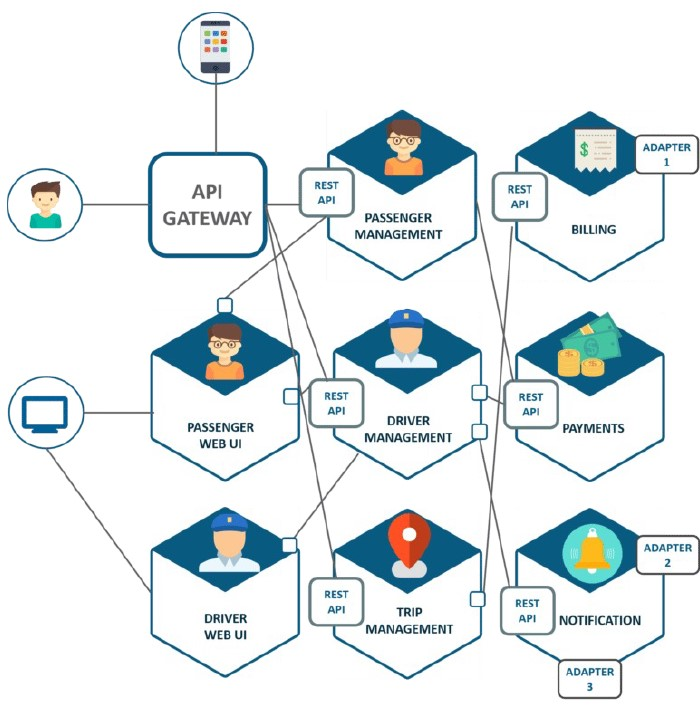
\includegraphics[width=0.8\textwidth]{img/ServicesComputing3.jpg}
\end{center}

\section{But… what is a “(Web) Service”?}
\underline{Informal definition}: A service is an independent software entity that can be discovered and invoked by other software systems over a network.
§ Definition from standardization body W3C (organo che gestisce le specifiche web, così dice CoPilot): A Web service is a software application
\begin{enumerate}
    \item identified by a URI (Uniform Resource Identifier),
    \item whose interfaces […] are capable of being defined, described and discovered […] and
    \item supports direct interactions with other software applications using […] messages via Internet-based protocols (di solito documenti in formato json, html, xml, etc\dots).
\end{enumerate}
A web service uses web technologies (especially HTTP) to provide functionalities. Non sono gli unici ma i più importanti in questo momento.
\\A me interessa sapere come è fatto un servizio, come invocarlo ed utilizzarlo.
\\Altre definizioni:
§ Web services are
§ self-contained,
§ self-describing,
§ modular applications that can be published, located, and invoked across the Web. (Tidwell, IBM, 2001)
§ Web services are
§ encapsulated,
§ loosely coupled Web “components” that
§ can bind dynamically to each other. (Curbera, IBM, 2001)

\section{Architectural building blocks}
Services are independent “components”
1. Well-known interface
2. Unique access point
3. Document-based data exchange
1. Well-known interface
§ Standard description language (e.g., WSDL) linguaggio usato per la definizione logica dell'interfaccia di un particolare servizio.
§ Possible automatic management by middleware

The term middleware is most used
for software that enables
communication and management of
data in distributed applications.

2. Unique \textbf{access point}
§ Use of URI (URL/URN)
§ Discoverable by means of name services (e.g., UDDI directory)

UDDI is an XML-based standard for describing, publishing, and finding web
services. UDDI stands for Universal
Description, Discovery, and Integration

3. \textbf{Document-based} data exchange
§ Use of standard representation format (e.g., XML, JSON)

\section{SOA core elements}
2 Componenti:
\begin{itemize}
    \item Service
    \item Service Description
\end{itemize}
Ruoli:
\begin{itemize}
    \item Service Providers: offer services/functionalities
    \item Service Brokers: menage service catalogs (i cataloghi dei servizi sono praticamente delle basi di dati in cui posso ricercare i servizi che meglio si adatta alle mie necessità fra tutti i servizi disponibili)
    \item Service Requestors: find a service and interacts with providers
\end{itemize}
Operazioni:
\begin{itemize}
    \item Publish (a service)
    \item Find (service/endpoint)
    \item Interact (e.g., request-response)
\end{itemize}
% image4

\section{Service Level Agreement (SLA)}
SLA is a contract between the provider and the user of the services.
\begin{itemize}
    \item Ensures that functionality is delivered correctly
    \item Non-functional properties
\end{itemize}
SLA (Service Level Agreement)
\begin{itemize}
    \item Defines the non-functional characteristics guaranteed by the service
    \item An SLA includes several SLOs (Service Level Objectives) that define the quality of service to be guaranteed through specific metrics
\end{itemize}
Ovviamente dire che un programma (Java) è corretto non basta per dire che sia utilizzabile: potrebbe essere troppo complesso o elaborato per essere riutilizzato.
% image

\section{Peculiarità dei Web Services}
Public components
§ “Discoverable” (naming, registries, accessing)
§ Public interfaces (standard protocols, machine handled)
§ Composability
§ Composite services: “orchestration”
§ Coordination: “choreography”
§ Semantic Descriptions
§ Discovery
§ Composition
§ Recommending Systems (in base alle parole che uso, mi consiglia servizi simili a quello che sto cercando)
§ …
§ QoS
§ Basic: security, availability, performance, …
§ Context awareness
§ …
§ System organization
§ p2p (any organization, application managed)
§ ESB (any organization, middleware managed)
§ Grid (given model) [a griglia]

Queste modalità rappresentano anche delle sfide.
\subsection{Challenges: how to do…}
Description
§ functional and QoS
§ Composition
§ orchestration
§ choreography
§ Semantic …
§ Infrastructure
§ Abstract/concrete architectural model
§ Services for services (servizi al servizio di altri servizi)
§ Service management
§ Global naming service
§ Software engineering
§ Development process
§ Deployment
§ Services for services
§ Global discovery service
§ Reputation
§ Transaction (workflow and exceptions)
§ Security
§ Monitoring (deve essere ben distribuito, visto che i servizi sono distinti)
§ Business
§ Business process support
§ Economic models
§ Organizational models

\section{Composizione di servizi}
What's a service composition?
§ A composition consists of a set of interconnected services, which may be used as a new service in other compositions
§ Two services are interconnected if at least one of the two requests the exposed functionality (a.k.a. endpoint a.k.a. API) of the other
Compatibility is required between interacting services for service composition to be successful
§ They must talk the same language (syntactically and semantically)
§ A service provider must present a published interface
\begin{center}
    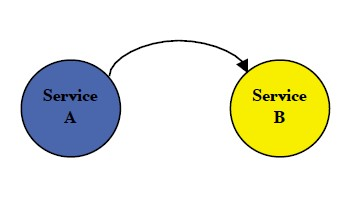
\includegraphics[width=0.375\textwidth]{img/ServicesComputing6.jpg}
\end{center}

\section{Business Processes}
Quando abbiamo tanti servizi, a livello aziendale possiamo pensare di metterli tutti assieme sullo stesso piano per riuscire a gestirli più facilmente. Parliamo di business process.
\\\underline{\textbf{Business Process}}: a set of related activities (workflow) performed by people and applications to achieve a well-defined business outcome (service or product).
\\Software BPs are created from the composition (integration) of services.
It may contain defined conditions triggering its initiation and defined outputs at its completion.
§ It may involve formal or relatively informal interactions between participants (humans and software).
§ It may contain a series of automated activities and/or manual activities.
§ It is distributed and customized across boundaries within and between organizations, often spanning multiple applications with different technology platforms.
§ It has a duration that may vary widely.
§ It is usually long running. A single instance may run for months or even years.

Dal punto di vista aziendale, per esempio questa parte del business process è affidata agli ingegneri del software.

\subsection{Software side: Orchestration vs Choreography}
\subsubsection{Orchestration}
describes how services interact with each other, including the business logic
and execution order of the interactions from the perspective and under the control of a single
actor (service).
§ For instance, there is orchestration when a service uses other services' functionalities (in the right
order) to implement its business logic
§ It requires active control. Cumbersome but easier to monitor.

\subsubsection{Choreography}
Interazione e cooperazione di tutti i servizi. Ogni servizio è consapevole di quale è la sequenza di invocazione degli altri servizi.
\\Describes the sequence of interactions among multiple parties involved in the process from the perspectives of all parties. It defines the shared state of the interactions between business entities.
\\Every service is responsible for completing its task also invoking other services. Usually implemented using events.

\section{Architetture orchestrate}
Molto semplici.
It is therefore possible to create a dynamic network of services, where individual services can be offered by
different organizations
§ One organization assumes the role of orchestrator and takes on the burden of implementing the controller
service for other organizations
§ There are usually organizations called service brokers.
§ Find the best alignment between services requested by Service Requestors and services offered by Service Providers
\begin{center}
    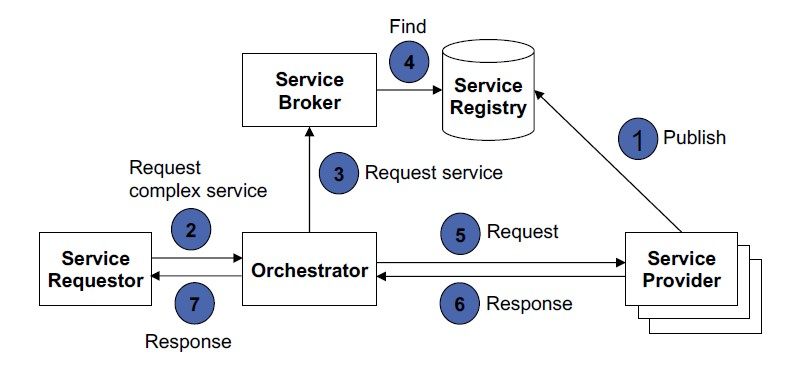
\includegraphics[width=0.5\textwidth]{img/ServicesComputing8.jpg}
\end{center}

\section{Enterprise Service Bus}
Pattern molto comune perché permette di facilitare l'integrazione fra applicazioni.
The SOA architecture has allowed the simplification of integration between the different components of an
information system
§ Exchangeable messages are defined a priori
§ It has led to the definition of the Enterprise Service Bus (ESB)
§ Communication system to support interaction and communication between components of an information system
§ Example of the choreographic approach
§ Usually implements the publish/subscribe pattern
§ Main Features
§ Message routing between applications and services
§ Message transformation
§ Secure communication
§ Extensible architecture
% image

\chapter{Soap Services}
\section{The Conceptual Web Service Stack}
A livello di rete, permette la comunicazione fra servizi in modo da rendere possibile il funzionamento dei servizi web.
\begin{center}
    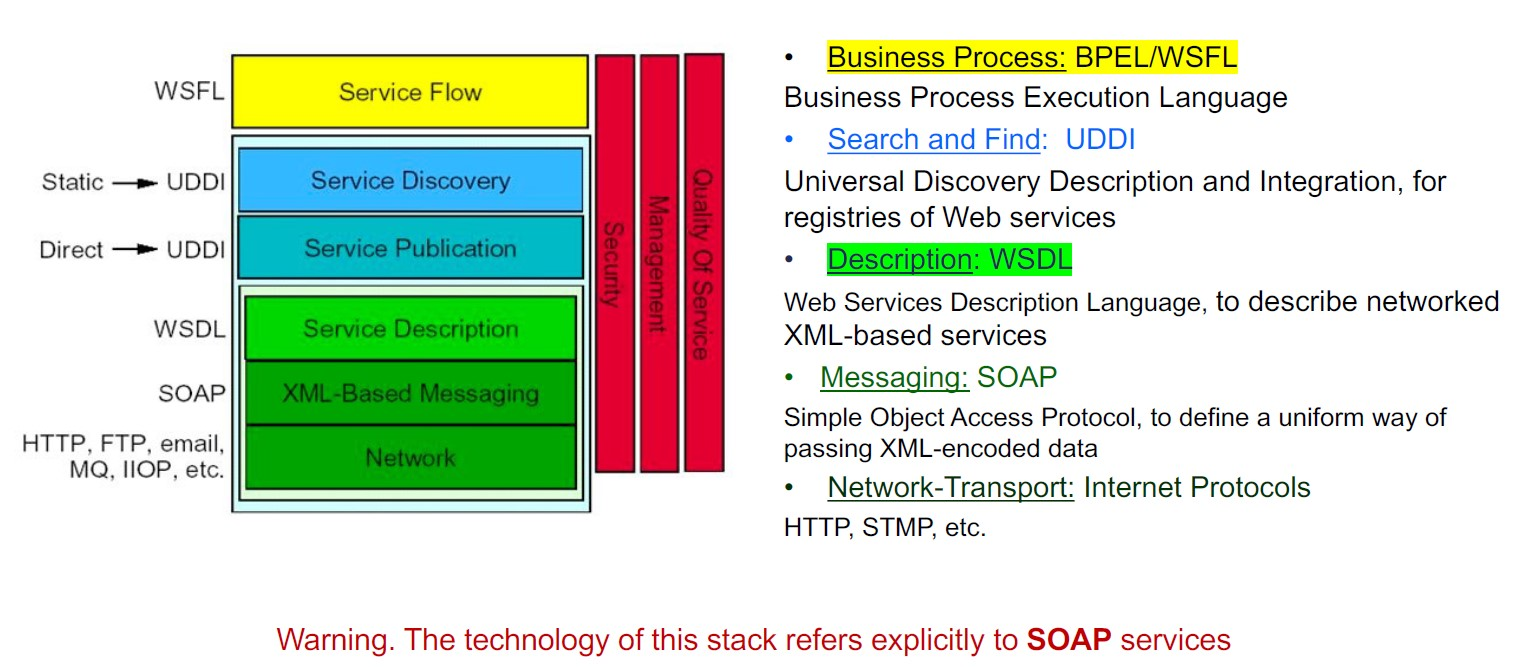
\includegraphics[width=0.5\textwidth]{img/SoapServices1.jpg}
\end{center}
Alla base di tutto questo meccanismo c'è il protocollo SOAP.

\section{SOAP: Simple Object Access Protocol}
SOAP is an XML-based protocol to let software components and applications to communicate using XML
messages
§ XML namespaces are used to provide semantics to data (not just data types)
§ It is agnostic of the transportation subsystem
§ Request and response messages
§ SOAP is a standard way to structure XML Messages (Data)
§ An application of the XML specification
§ Relies on XML Schema, XML Namespaces
§ It is not tied to any programming language or platform (not even to web services)
§ Simple and extensible
§ Used in document-oriented services, ovvero c'è scambio di informazioni in formato testuale (se non fosse orientato a documenti, a cosa potrebbe essere orientato? Una possibilità sarebbero le chiamate a procedura remota, hanno la struttura di una funzione e l'unica cosa che c'è bisogno di fare è definire il nome e i parametri di I/O).
\begin{center}
    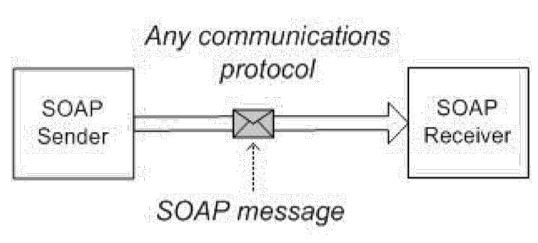
\includegraphics[width=0.5\textwidth]{img/SoapServices2.jpg}
\end{center}

\subsection{Componenti di un messaggio SOAP}
\subsubsection{SOAP Envelope}
Wraps the contents of the message
\subsubsection{SOAP Header (opzionale)}
More flexibility, can be processed by nodes between the source and destination
\\Contains blocks of information regarding how to process the message:
\\Routing and delivery settings
\\Authentication/authorization assertions
\\Transaction contexts
\subsubsection{SOAP Body}
Actual message to be delivered and processed
\\Both for request and response information
\begin{center}
    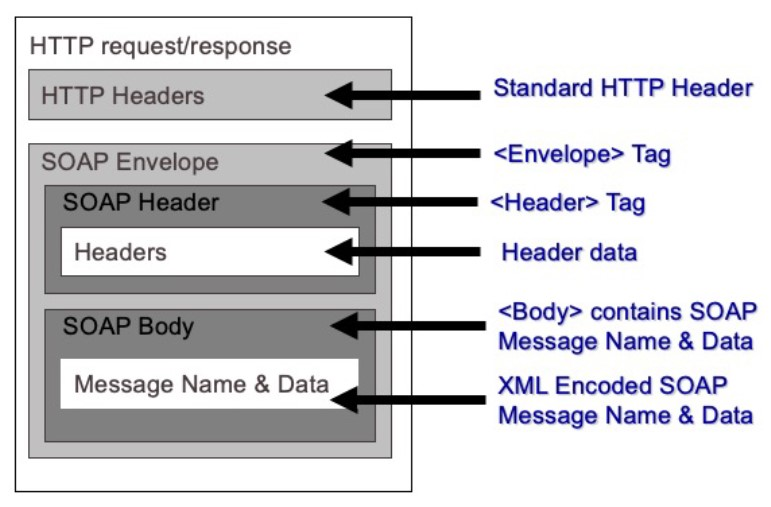
\includegraphics[width=0.5\textwidth]{img/SoapServices3.jpg}
\end{center}
In questo esempio il messaggio SOAP è composto come un payload di un messaggio HTTP.

\subsection{SOAP with HTTP}
Although SOAP can use several transport protocols, HTTP is the one most commonly used.
§ HTTP requests consist of an HTTP, such as POST or GET, followed by the URL requested and the protocol
version (e.g. HTTP 1.1).
§ Responses follow the semantics of HTTP to provide the status code of the response;
§ For example, a status code of the type 2xx indicates that the request has been received, understood, accepted, etc.
There are two models for exchanging messages SOAP via HTTP (è necessario che il client sia quello che per primo crea la comunicazione):
§ the "SOAP request-response" model in which the POST method is used to bring SOAP messages into the body of
the http requests/responses;
§ the "SOAP response" model in which in http requests is used the GET method to get the SOAP message and insert
it into the Body of the response.
§ Using SOAP with HTTP one must remember to set the Content-Type header as application/SOAP+xml

\subsubsection{examples:}
% due images

\section{WSDL}
Linguaggio basato su XML pensato per descrivere l'interfaccia di un servizio web.

\subsection{What is WSDL?}
§ Web Service Description Language (It is pronounced [wizdel])
§ Used to define “How and where to access the service”
§ XML-Based Language for describing web services, the messages and how to invoke them
§ A WSDL file contains a description of a service’s interface
§ WSDL allows to describe four main pieces of data for a service:
§ Interface information describing all publicly available operations of a service
§ Data type declarations for all messages. Complex types can be declared (using SOAP) and used
§ Binding information about the transport protocol (HTTP, SMTP, UDP)
§ Address information for locating the service (URI)
§ Abstract vs. concrete services
§ WSDL is a W3C Recommendation
§ WSDL 2.0 became a W3C Recommendation 26 June 2007

\subsection{WSDL 2.0: conceptual model}
In the abstract part
§ Description of a web service in terms of messages it sends and
receives through a type system, typically W3C XML Schema
§ An operation associates message exchange patterns with one
or more messages
§ Message exchange patterns define the sequence and
cardinality of messages exchanged between nodes (services)
§ An interface groups these operations in a transport and wire
independent manner

In the concrete part
§ Bindings specify the transport protocol for interfaces
§ An endpoint associates a URI with a binding
§ A service groups the endpoints that implement a common
interface
% image

\subsection{WSDL 2.0: definizione di binding}
\subsubsection{Binding}
The name attribute defines the name of the binding. With this name you can reference it when defining a service endpoint. Every binding name must be
unique within the WSDL 2.0 target namespace.
The interface attribute contains the name of one of the defined interfaces
The type attribute defines which message format is to be used. In this case is SOAP (other bindings are possible).
wsoap:protocol defines the “transport” protocol. In the example, soap messages are going to be transported using HTTP
\begin{center}
    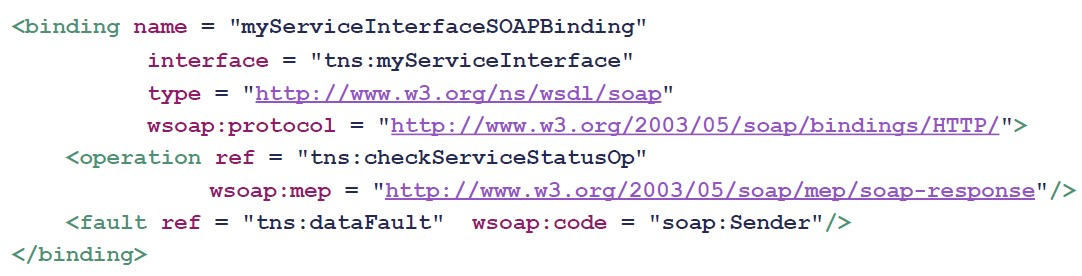
\includegraphics[width=0.5\textwidth]{img/SoapServices7.jpg}
\end{center}

\subsubsection{Operation}
The ref attribute of the operation element references a specific operation (already defined in the interface section)
The wsoap:mep attribute defines the message exchange pattern for SOAP (GET request)

\subsubsection{Fault}
The ref attribute defines which fault (already defined in the interface section) will be referring
The wsoap:code attribute of the fault element defines the fault code that will trigger sending this fault message

c'è una slide 

\section{Perché non si usa più - Why SOAP dream faded away}
The stack of protocols collapsed under its own weight
§ WSDL and SOAP are too verbose, hard to understand, complex
§ A more simple and readable approach was felt necessary
§ Agreed upon semantics for method and JSON for the payload
§ DNS, human-readable names for endpoints
§ A new (fun) kid in town: REST

Troppo preciso, troppo pedante, troppi riferimenti a XML. Ci sono ancora molti servizi che usano questa tecnologia, ma quelli nuovi difficilmente lo usano.